\chapter{Methodology}

\section{Introduction}

In order to characterise the synthesised materials and acquire information about the chemistry, crystallinity, morphology as well as its optical and electrical properties a suite of state of the art techniques has to be utilised. An overview of those techniques has been provided in theory and experimental setup.

\section{Raman spectroscopy}

Raman spectroscopy is one of the most useful and versatile characterisation techniques for 2D TMDCs due to its non destructive and ease of use. The lack of need to extensively prepare the sample like in some other techniques allows for relatively fast measurements of a large number of samples. Additionally the lack of transfer required results in minimal changes to to the material itself as well allows for easier tracking of specific areas of the sample across different techniques. Raman spectroscopy can be used to measure as grown by CVD samples on $Si/SiO_2$ substrate or any other solid substrate as well as liquid solution samples produced by liquid exfoliation.

The Raman spectroscopy can be used to extract information about the chemistry of the material as well as the crystal structure, the number of layers of 2D TMDCs or the strain within the layers. 

When a material is irradiated with light the photons generally scatter at different angle but same wavelength. However certain small part of the incident photons (about 1 in 10 million) is scattered at different wavelength than the incident one. This is known as the Raman effect and the photons that are scattered at wavelengths greater than the incident ones are due to Stokes scattering, while the ones emitted at wavelengths smaller than the incident one are due to anti-Stokes scattering. In the Stokes scattering phenomena the phonon is emitted while during the anti-Stokes scattering the phonon is absorbed as seen in Figure \ref{fig:MethodologyRamanEnergyLevels}. In order for the Raman effect to take place a transition between two resonant states must occur. The probability of transition from lower to higher energy state depends on the population of the states. In a thermodynamically stable system the lower energy states are more occupied than the higher energy and therefore the transition from lower to higher is more likely to occur (Stokes scattering). The spectrum of photons scattered as a result of Raman scattering forms what is known as Raman spectrum, where the number of photons scattered is plotted against the photon frequency difference between the incident and the scattered photons. The spectrum is symmetrical around the spectrum origin in regards to the frequency but not in terms of intensity. Because of that only the Stokes part is generally used as a Raman spectrum.

\begin{figure}[!h]
	\begin{center}
		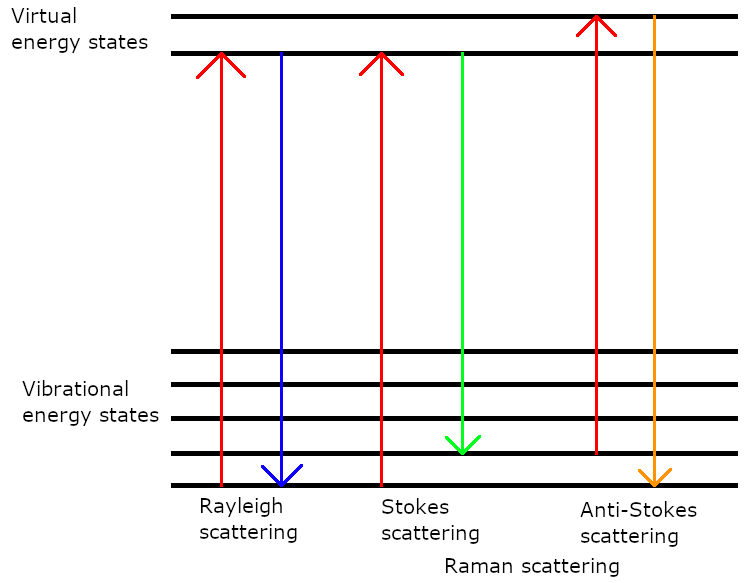
\includegraphics[scale=0.3]{Methodology/RamanEnergyLevels.png}
		\caption{An energy diagram comparing elastic and inelastic scattering. Reproduced from en.wikipedia.org}
		\label{fig:MethodologyRamanEnergyLevels}
	\end{center}
\end{figure}

The phonons that are emitted or absorbed during the transitions between the virtual states in the Raman effect are phonons of the vibrational modes in the material. For any solid state crystalline material the point group can be defined. Using the point group the available vibrational modes can be found. In order for Raman scattering to occur a change in polarisability must occur in a given vibration mode. Similarly if the vibrational mode results in change in dipole moment it results in an IR active mode. As a result a set of available Raman active modes can be found. The Raman spectrum can be therefore used to identify the vibrational modes and therefore gain insight about various factors that influence those vibrational modes.

A typical Raman spectroscope setup involves a monochromatic light source, generally a laser, which is focused on a sample. As a result some of the light is scattered elastically (Rayleight scattering) while even smaller part is scattered inelastically (Raman scattering). The scattered light is then passed through a filter to remove the elastically scattered light at the wavelength equal to that of the incident photons. The remaining Raman scattered light is passed through a monochromator and then onto a CCD detector. A diagram of a Raman spectroscope can be seen in Figure \ref{fig:MethodologyRamanSetup}.

\begin{figure}[!h]
	\begin{center}
		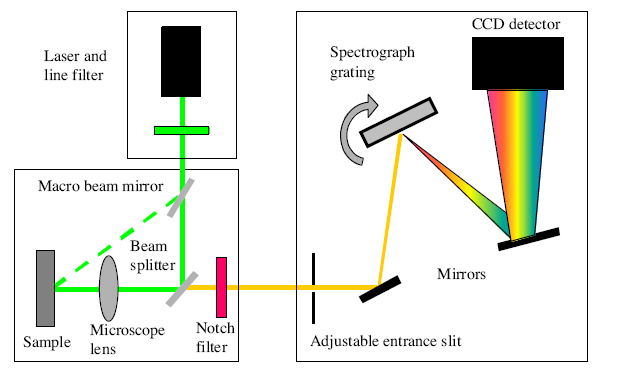
\includegraphics[scale=0.7]{Methodology/RamanSetup.png}
		\caption{A typical Raman spectroscope setup. Reproduced from www.sas.upenn.edu}
		\label{fig:MethodologyRamanSetup}
	\end{center}
\end{figure}

A Raman spectrometer used in this work is a Renishaw Raman spectrometer. The 532nm laser was used as a light source in a backscattering geometry. Unless otherwise specified the measurements were taken at room temperature and ambient pressure. An objective lens of 100x with 0.9 numerical aperture was used as the focusing lens. The laser power was set to be 1.6mW with 0.1s acquisition time for mapping and 1s acquisition time for single spectra. The grating of 1800 lines/mm was used resulting in a resolution of about 1.5 $cm^{-1}$. For calibration purposes a silicon sample was used with a peak at 520 $cm^{-1}$. All data analysis was performed using MATLAB software. The peak fitting script used has been attached in Appendix \ref{app:Matlab}.

\section{Photoluminescence spectroscopy}

The photoluminescence spectroscopy (PL) is an another versatile non-destructive characterisation technique. When applied to the 2D TMDCs it can provide great insight into the crystal stricture, electronic structure of the material as well as some direct information about its optical properties. One of the great advantages of PL spectroscopy is shared with the Raman spectroscopy in that the sample preparation and handling is very easy and quick allowing for high throughput of characterisation. Unlike Raman spectroscopy a substrate choice might become more important for PL measurements owing to the fact that the conductive substrate might result in PL quenching. Since the bandgap of many of the 2D TMDCs lies within the optical range of the spectrum or near to it a single laser at 532nm can be used to excite the samples.

Photoluminescence is a type of luminescence where an excitation is provided by the incident light. 

\section{X-ray photoelectron spectroscopy}